\documentclass[UTF8]{article}
\usepackage[a4paper, total={6in, 8in}]{geometry}
\usepackage{enumitem}
\usepackage{graphicx}
\begin{document}

\title{%
    COMP 8920 - Computational Reasoning in AI \\
  \large Literature Review - Submission 2\\}

\author{%
    Vijay Rajasekar Thirulokachander\\
    105092311\\
    \large thirulo@uwindsor.ca}
\date{}
\maketitle

\section{Introduction}
This literature survey focuses on research that uses Subjective Logic to deal with uncertainty in the domain of argumentation. 
In Section 2, we review the work of F. Santini et al. in \cite{8455455}, which explores the use of Abstract Argumentation Frameworks (AAFs) to help agents determine whether an argument or attack 
is trustworthy and provide a new approach to the use of AAFs with Subjective Logic. Section 3 reviews the work of A. Koster et al. in \cite{Koster2017} on the use of Belief Revision operators. 
N. duy Hung in \cite{8023355}, evaluates the use of Probabilistic Assumption Based Argument Frameworks which is reviewed in Section 4.  In Section 5, the concept of 
dialogue based information exchange in argumentation using sensors by N. Oren in \cite{OREN2007838} is surveyed. Finally, in Section 6, we take a look 
at the work of A. Groza et al. in \cite{8516616} for a practical implementation of subjective logic in argumentation, by determining the acceptability of arguments related to climate change denial.

\section{Are my arguments trustworthy? Abstract argumentation with Subjective Logic}
\subsection{Problem Addressed}
P. M. Dung's Abstract Argumentation Frameworks\cite{DUNG1995321} proved to be an effective method for the 
representation of arguments and conflicts expressed in natural language. However, these frameworks ignore any 
relationship between the arguments in conflict. Arguments can be fallacious due to the presence of enthymemes, 
wherein a premise is not stated, thereby leading to uncertainty of trustworthiness. 
Furthermore, due to characteristics of natural language, the attack of one argument upon another may not be present at all, but an agent may interpret it as one. 

\subsection{Previous work by others that attempted to solve the same problem}
E. Dunne et al. introduced the concept of weighted arguments in \cite{DUNNE2011457}, which uses a characteristic referred to as an inconsistency budget
that determines how much inconsistency the AAF can tolerate. The authors of \cite{8455455} draw a parallel between the use of weights and the use of subjective beliefs as the latter being a different interpretation of the former.

S. Bistarelli et al. in \cite{Bistarelli}, pointed out the drawbacks in \cite{DUNNE2011457} and the possibility of a ripple effect arising due to a minor conflict in arguments, which may adversely affect the
strength of a defense. To address this issue, the authors use a commutative semiring structure to implement new weighted notions that effectively provide relaxation to the approach used in \cite{DUNNE2011457}, 
thereby improving the quality of solutions offered by the agent, and reducing the effect of noise generated by harmful elements(trolls) in an abstract framework.

The authors of \cite{8455455} also speak briefly about the concepts implemented in \cite{Koster2017} and \cite{OREN2007838} and the difference between the scenarios that the concepts are targeted towards concerning \cite{8455455}. 
These papers will be reviewed at length in Sections 3 and 4.

\subsection{Shortcomings of previous work}
The authors do not point out any drawbacks in the approaches taken by the authors of the abovementioned papers but rather refer to them as varied approaches to tackling uncertainty and subjective belief in AAFs.

\subsection{Description of the Proposed Approach}
The authors improve upon a Constellations approach defined in \cite{dung2010towards} that assigns a probability distribution 
over argument sets. 
They replaced the probability distribution with Subjective Logic since SL provides a mechanism to take uncertainty into account. An AAF that
uses Subjective Logic is defined by the authors to be an slAAF. 

\subsection{Analysis and Experimentaion of the Proposed Approach}
The paper measures the impact of subjective opinion on the parameters required for an argument to be considered an \textit{Accepted Argument} viz. conflict-free sets, admissible sets, complete semantics, preferred semantics
and stable semantics. An AAF consisting of arguments that can be considered Accepted Arguments can be induced from an slAAF if it satisfies the 
following criteria:
\begin{itemize}
  \item The set of arguments in the AAF is a subset of the arguments in the slAAF,
  \item The attacks in the AAF are a subset of the intersection of the set of attacks in the slAAF with the Cartesian product of the set of induced arguments with itself,
  \item For every argument in the set of arguments in the slAAF, the belief score is 1.
  \item For every attack between two arguments in the slAAF, the belief score is 1.
\end{itemize}
In the induced AAF, the set of here is no evidence of impact at the time of writing this literaturesurvey
arguments consisting of enthymemes and fallacies are assigned a belief score of lower than 1 and an uncertainty score greater than 1. The sum of all expectation values of all the AAFs that can be induced from an slAAF is 1.

The authors also analyse different approaches towards fusion of subjective belief in the Constellations approach. \textit{Averaging Fusion} is used for fusing beliefs over a set of arguments in an slAAF.

\subsection{Results that the authors claim to have achieved}
Since this paper focuses more on defining Subjective Logic operations, operators, and criteria for its application in argumentation and less on experimentation, no concrete results are mentioned by the author.

\subsection{Claims made by the authors with respect to their contribution}
The authors explain their reasoning behind the use of subjective logic in Constellaion AAFs and how it can be used to determine trustworthiness
of arguments. In the future, they intend to bring a similar approach to Epistemic AAFs, in which an agent is less likely to believe in an attacking argument, 
if its belief in the defending argument is higher. They also intend to use Subjective Logic to perform ranking of arguments by 
computing the effect of each argument upon the other.

\subsection{Citations to the paper by other researchers}
Searching for citations to this paper on Google Scholar and Scopus archives did not yield any results. This could be attributed to the fact that this paper was published just eight months before this literature survey was written.

\subsection{Evidence of impact of the paper}
After a thorough look through Google Scholar, Scopus and ResearchGate, it is safe to say that there is no evidence of impact at the time of writing this literature survey. Since the implementation of Subjective Logic in argumentation is an ongoing research topic, there is a possibility that researchers working in this topic will be citing this paper due to Prof. Josang's contributions to this field.

\section{Liar liar, pants on fire; or how to use subjective logic and argumentation to
evaluate information from untrustworthy sources}

\subsection{Problem Addressed}
The authors approach the conflict of arguments and information in a system where communication between agents plays
a major role in the functioning of the system. The system has to decide which agent is providing more trustworthy information
and the revision of belief based on trustworthiness. 
An example of such a system in which the authors implement their approach 
is that of a collaborative traffic information application. 

\subsection{Previous Work}
The authors describe the similarity and differences between their work and that of Tang et al. in \cite{Tang2012UsingAT} regarding belief revision, wherein the update of information is considered
to be only from a single source and the lack of a mechanism to deal with similar propositions from multiple agents. 

The work of Pereira et al. in \cite{Pereira} uses possibilistic logic in belief revision. In this approach, if there are multiple 
trustworthy agents that provide conflicting information to each other, the system believes in neither agent.

\subsection{Shortcomings of previous work}
The authors state that most of the related work in the domain of belief revision lack proper treatment of aggregation of credibility 
of various sources that contribute information, based on the trustworthiness of each source. They point out that the establishment of a 
predetermined ordering of belief change in 
the work of Falappa et. al in \cite{Falappa} is based on a confidence level which is not updated with a change in trustworthiness of the agent.

\subsection{Description of the Proposed Approach}
To overcome the drawbacks of the approaches in \cite{Falappa} and \cite{Tang2012UsingAT}, the authors proposed a new type of Belief Change Operator. 
The agent receives information in two forms: large amount of conflicting data, and a belief change operator that includes subjective logic
into an argumentation framework to make the agent provide higher importance to some part of the conflicting data over the rest. The authors use 
the argumentation framework suggested by Amgoud and Vesic in \cite{AMGOUD2014585} as they believe it provided a better way of representing preference
ordering using subjective logic compared to Dung's \cite{DUNG1995321} AAF model.

The authors detail a set of specifications that determine how an agent's beliefs are computed based on received information. These are defined as follows:

\begin{enumerate}
  \item Information collection
  
  A trust model is used to determine how trustworthy a source is and how credible the information provided by the source is. The authors claim that 
    most belief revision operators do not focus on this step as much as they do on deciding what information to believe in.

  
  \item Aggregation of Information
  
  To combine the opinion of different opinions of the same proposition, the cumulative fusion operator
  is used.

  \item Selection of Information to believe in
  
  On a set of Arguments that can be generated from a set of Propositions a resulting base belief set is obtained. We provide a 
  preference relation to this set. A tuple consisting of a set of arguments, the relationships between these arguments, and the preference ordering 
  of these arguments acts as the Belief Change Operator.

  
\end{enumerate}

\subsection{Analysis and Experimentaion of the Proposed Approach}
The authors conduct two sets of experiments to determine the effectiveness of using belief revision
in a collaborative agent-based traffic model. Two paths are presented from a source to a destination 
on a map. The agents receive information that one path is longer than the other. However, the shorter 
path is considered to be dangerous according to the beliefs of other people. Therefore, more people choose to
take the longer route which ends up being congested. 

In the first experiment, the agent runs for 100 iterations. Various levels of trustworthiness are applied to different sources
of information received about the dangerousness of the shorter path which affects the agent's choice to 
decide on a route. 300 agents are used in total, of which a major part are classified as private drivers, 
and the rest are divided into professional drivers and authority drivers. A certain percentage of each class 
of drivers are also considered to be liar agents. Sometimes, information is not broadcast to all of the agents in the experiment. The ability of each agent to update its belief based on the 
various sources of information it receives is analysed.

\subsection{Results that the authors claim to have achieved}
The authors observed that when all the agents have perfect information about the dangerousness of the shorter path, 
they chose it over the longer path. When a small amount of discomforting information is provided, the randomness in choice
of paths increases when using possibilistic logic. However, in the subjective logic based framework, the authors noted that 
belief revision occurs properly and the agents make the right choice to follow the shorter path. 

When both liar agents and information broadcast were added, the belief revision operator helped 
agents filter out untrustworthy information over time and in the end, all the agents ended up choosing the shorter path.

\subsection{Claims made by the authors with respect to their contribution}
The authors claim that their Belief Revision Operator performs as well as existing models, if not better.
They point out that the performance of the approach taken by Pereira et al. is much poorer than theirs due to the lack of a robust framework.

The authors plan to explore the use of their Belief Revision Operator when false institutional memory is present in a social environment.  

\subsection{Citations to the paper by other researchers}
This paper has been cited by Prof. Josang in \cite{8455455} regarding its use of belief operators based on SL operators and how they intend to apply this approach alongside their implementation of SL in Abstract Argumentation Frameworks.

\subsection{Evidence of impact of the paper}
According to ResearchGate, this paper has been cited in three different works, one of which is Prof. Josang's \cite{8455455} as mentioned above. Google Scholar mentions an additional citation in a paper studying Enthymemes in multi-agent systems.

\section{Probabilistic Assumption-based Argumentation with DST evidence}
\subsection{Problem Addressed}
The author tackles the mathematical inequivalence of Dempster Shafer Theory and Probabilistic Assumption-based Argumentation(PABA) to demonstrate the need for an argumentation framework in a scenario where DST based evidence is insufficient. 

\subsection{Previous work by others that attempted to solve the same problem}
The work of Kohlas et al. in \cite{Kohlas2002} to associate probability 
mass to compute belief measures is noted by the author. He highlights the efforts of Samet et al. in \cite{10.1007/978-3-319-40581-0_21} to use DST to describe the uncertainty regarding different versions of the same argument. He also details the work of various authors on the combination of argumentation with probability theory to propose different Probabilistic Argumentation frameworks.

\subsection{Shortcomings of previous work}
The author mentions that work of Kohlas et al. in \cite{Kohlas2002} is limited by its ability to function only with conjunctions of literals. 
\subsection{Description of the Proposed Approach}
To study the relationship between a PABA framework and DST based evidence, the author uses the PABA model proposed in \cite{Dung:2010:TAJ:1860828.1860846}.   The criteria for a PABA framework to be considered a relatively grounded framework is applied to the PABA representing DST evidence and is proven. Then the author proceeds to define DST belief and plausibility degrees in PABA semantics.

\subsection{Analysis and Experimentaion of the Proposed Approach}
To demonstrate the relationship, 
the author shows that each DST body of evidence can be represented by a PABA framework wherein grounded semantics and credulous semantics are mapped to DST belief and plausibility functions. The mass functions are 
constructed in the form of a PABA network.
\subsection{Results that the authors claim to have achieved}
The author shows that each DST body of evidence can be represented by a PABA framework whose grounded semantics and credulous semantics respectively coincide with DST belief
function and plausibility function. He also claims that DST rules for combining independent bodies of evidence are instances of a canonical rule for combining PABA frameworks.

\subsection{Claims made by the authors with respect to their contribution}
The author details the possible application of PA frameworks in many practical scenarios involving 
DST and claims that this paper will appeal to a large community of DST users. He also claims that DST is limited in the approach towards a unified theory of logical and probabilstic reasoning.

\subsection{Citations to the paper by other researchers}
Searching for citations to this paper on Google Scholar and Scopus archives did not yield any results.
\subsection{Evidence of impact of the paper}
On ResearchGate, this paper is listed under an ongoing project: \textbf{\textit{Probabilistic Argumentation}} by the author. At the moment of writing this literature review, no evidence of significant impact of this paper could be found.

\section{Subjective logic and arguing with evidence}
\subsection{Problem Addressed}
The authors attempt to address situations consisting of different agents that are trying to reach a shared conclusion about a particular state of the environment 
they are present in. Various assumptions are made, such as: 
\begin{itemize}
  \item the information obtained through sensors could potentially be wrong, 
  \item some subsets of the environment are observable
  \item agents are self interested and may have opposing goals 
\end{itemize}

\subsection{Previous work by others that attempted to solve the same problem}
The authors mention the work of Pollock in \cite{Pollock:1995:CCB:526901} towards the use of probability in argumentation frameworks. They also mention the use of evidence based argumentation in Haenni \cite{Haenni2005TowardsAU} and how he shows a relation between his work and Dempster-Shafer Theory.

\subsection{Shortcomings of previous work}
The authors point out the weaknesses in the probabilstic approaches mentioned above concerning the construction of evidence based argumentation frameworks as they perform 
inference when faced with uncertainty and conflicting arguments. 

\subsection{Description of the Proposed Approach}
The authors identified the need for four layers of an argument framework to have agents engage in dialogue 
and obtain shared information from different sensors to construct a shared world view. These layers are implemented as below:
\begin{itemize}
  \item Logical Layer: Built using Subjective Logic as proposed by Prof. Josang
  \item Dialectic Layer: Construction of arguments and represent the accrual of arguments and argument schemes
  \item Procedural Layer: Sensors to capture environment information
  \item Heuristic Layer: Provides decision making capabilities for the agents to decide on which sensors to use for probing
\end{itemize}

Across multiple layers of the framework, instances of arguments are represented in the form 
of tuples comprised of a set of Possible Facts about the universe associated with the environment and a set of Argument Schemes.

\subsection{Analysis and Experimentaion of the Proposed Approach}
An example consisting of two agents and a set of argument schemes is set up with the intent to determine the amount of building materials required. Agent $\alpha$ is 
assigned to be responsible for the stock and supply of steel, whereas $\beta$ is responsible for the supply of concrete. Both agents have self-serving (opposing) 
agendas in the same environment - to minimize the amount of their corresponding building material used in the bridge.

A set of argument schemes consisting of the various requirements that each material must satisfy for its use is defined. On experimentation, a dialogue takes place 
between the two agents by each probing a different sensor of the other to see if the building conditions are satisfied in a manner most suitable to its 
own goal. To tackle uncertainty of any sensor, belief opinions are used. As the dialogue proceeds, each agent accrues a set of arguments that assign an opinion 
value to its base predicates.

\subsection{Results that the authors claim to have achieved}
The authors observed that both agents agreed to come to a solution that satisfies their self serving goals. Through repeated probing of sensors and 
handling of uncertainty, arguments were accrued in favor of one agent. Fig. \ref{fig:fig1} represents the dialog that took place between the two agents and the probing of various sensors.

\begin{figure}
  \centering
  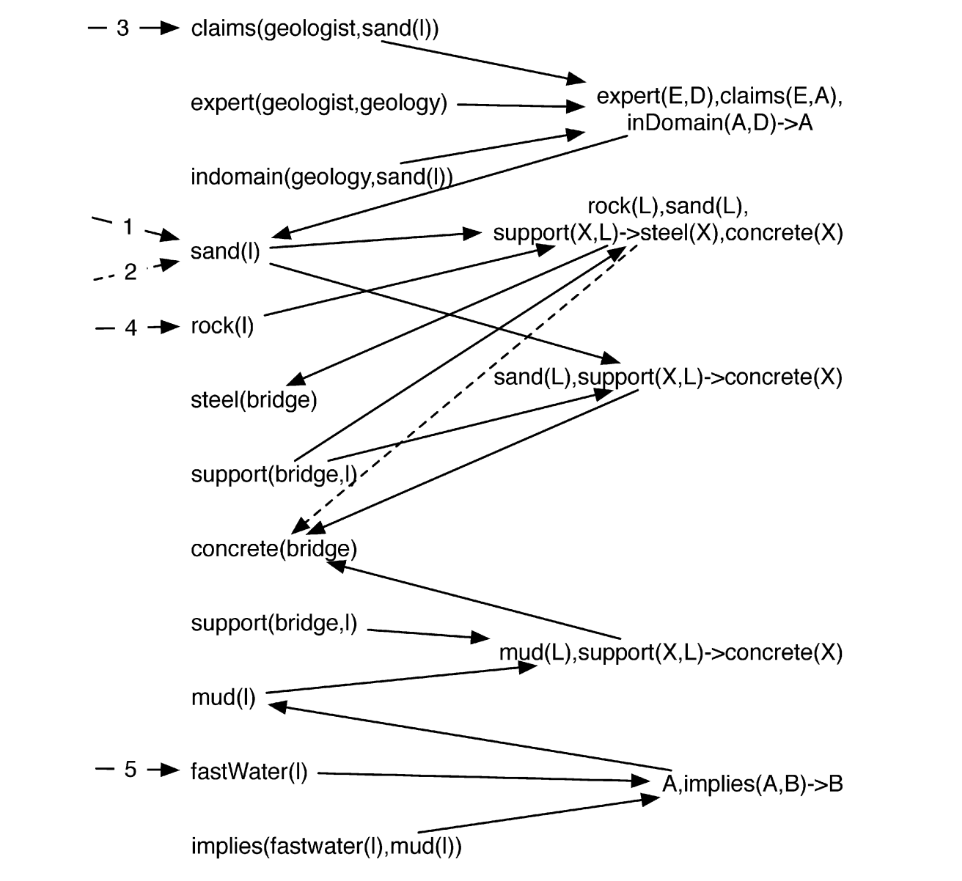
\includegraphics[width=10cm]{dialog}
  \caption{Dialog Argument Graph between the two agents. Image taken from \cite{OREN2007838}.}
  \label{fig:fig1}
\end{figure}

\subsection{Claims made by the authors with respect to their contribution}
The authors claim that the model is general enough to be applied to almost any area in which argument is employable. However they also state that 
this applies only to the lower levels of the model, whereas the higher levels require evidence based reasoning. In the future, they aim to enrich the sensor model 
in order to provide better opinions on information as well as to achieve a mapping between dialogue based argument framework and Dung's argumentation Framework \cite{DUNG1995321}.

\subsection{Citations to the paper by other researchers}
\begin{itemize}
  \item Groza et al. \cite{8516616} cite the approach taken in this paper towards belief updation. This paper will be reviewed at length in Section 6.
  \item Josang et al. \cite{8455455} cite how this paper details the construction of an argumentation framework intended for evidential reasoning, but mentione that this paper deals with structured argumentation, while their work deals with abstract argumentation. This paper was reviewed in Section 2.
\end{itemize}

\subsection{Evidence of impact of the paper}
According to ResearchGate, this paper has been cited 37 times. These citations are spread across various domains such as blockchains, bayesian trust modelling etc.  

\section{Analysing climate change arguments using subjective logic}
\subsection{Problem Addressed}
The authors attempt to analyse various arguments on the issue of climate change, obtained from online debate websites. However, when dealing with a large amount of 
collective opinion, an aggregation of arguments is required to obtain a top-level view of people's beliefs.
\subsection{Previous Work}
To analyse trust networks, the authors cite the approach taken by A. Josang et al. in \cite{Jsang2006TrustNA} using subjective logic. In this approach, the trust in the overall system 
is measured based on trust between each agent. They also cite the work of N. Oren et al. in \cite{OREN2007838} and draw similarities to their approach which includes belief and ignorance. 

\subsection{Shortcomings of previous work}
The authors point out that the approach taken in 
\cite{OREN2007838} focuses on the constant updation of accrued beliefs and arguments, whereas their approach deals with aggregation of arguments.

\subsection{Description of the Proposed Approach}
The authors constructed a corpus of arguments from three debate sites to evaluate the binomial opinion on user posted topics/hypotheses. A \textit{collective opinion} 
parameter is defined by the authors as a binomial opinion on a given hypothesis $h$, represented as a quadruple consisting of the belief value, disbelief value,  the ignorance degree, 
and the prior information available on that topic. The collective opinion on each hypothesis is measured across different communities of users, with care taken to avoid accidental duplicate 
arguments posted by users. Furthermore, a consensus operator is defined by the authors to help aggregate opinions across communities.

The potential of clustering the hypotheses is identified and its use in determining ignorance levels is measured. To cluster hypotheses, an Affinity Propagation algorithm \cite{Frey972} is implemented by the authors.

\subsection{Analysis and Experimentaion of the Proposed Approach}
The authors observed that upon aggregation of opinion on higher number of arguments, a consensual opinion had 
lower ignorance levels, therefore resulting in higher confidence levels on a given set of hypotheses. This operator also helps determine if 
an entire community is in support of a certain hypothesis by ranking the computed distance of opinions between two communities.


\subsection{Results that the authors claim to have achieved}
The authors claim that a low level of ignorance is the result of a large number of arguments being posted about this topic, which means there is a high level of interest for that topic. 
The ignorance level helped measure the expectancy of any given argument to be considered an \textit{accepted argument}.

Upon analysis of the clustered hypotheses, the authors note that out of 193 clusters, only one cluster had a balanced score in favour of a higher disbelief degree for the hypothesis:
 \textit{Developed countries should have a moral obligation to mitigate the effects of climate change}, as well as the lowest ignorance score.
\subsection{Claims made by the authors with respect to their contribution}
The authors claim that their approach for analysing people arguments can be applied in different domains, other than the one exemplified in the paper, i.e. climate change.

\subsection{Citations to the paper by other researchers}
Searching for citations to this paper on Google Scholar and Scopus archives did not yield any results. This could be attributed to the fact that this paper was published about six months before this literature survey was written.

\subsection{Evidence of impact of the paper}
On ResearchGate, this paper is listed under an ongoing project: \textbf{\textit{Increasing understanding on climate change through public discourse analyse and stakeholders modelling}}. According to the project description, the authors are attempting to facilitate understanding of controversial topics related to climate change as reflected in the public arena by different stakeholders and representing the justifications of opinions and their trends. This paper may have significant impact on this project in the future, but there is no evidence of impact at the time of writing this literature survey.

\section{Conclusion of Survey}
In this literature survey, we have looked at various approaches towards the implementation of subjective logic and belief theory in argumentation. We explored the use of Abstract Argument Based Frameworks and Structured Argument Based Frameworks, and we looked at an implementation of such an AAF on a real-time debate forum. A majority of the papers that were surveyed are from the past 2 years. 
Therefore their impact in related research hasn't been very profound at this moment in time.
\bibliography{LiteratureSurvey}{}
\bibliographystyle{ieeetr}
\end{document}